% Template:     Informe/Reporte LaTeX
% Versión:      2.2.6 (22/10/2016)
% Codificación: UTF-8
%
% Autor: Pablo Pizarro R.
%        Facultad de Ciencias Físicas y Matemáticas.
%        Universidad de Chile.
%        pablo.pizarro@ing.uchile.cl, ppizarror.com
%
% Licencia: CC BY-NC-SA 4.0 [http://creativecommons.org/licenses/by-nc-sa/4.0/]
% Sitio web del proyecto: http://ppizarror.com/Template-Informe/

% CREACIÓN DEL DOCUMENTO, FUENTE E IDIOMA
\documentclass[letterpaper,12pt]{article}  % Articulo tamaño carta, fuente de 11pt
\usepackage[utf8]{inputenc}                % Codificación UTF-8
\usepackage[T1]{fontenc}                   % Soporta caracteres acentuados
\usepackage{lmodern}                       % Tipografía moderna
\usepackage[spanish]{babel}                % Define el idioma del documento en español



% INFORMACIÓN DEL DOCUMENTO
\newcommand{\nombredelinforme}{Proyecto Speed dating}
\newcommand{\temaatratar}{¿Es posible encontrar el amor en 4 minutos?}
\newcommand{\fecharealizacion}{\today}
\newcommand{\fechaentrega}{\today}

\newcommand{\autordeldocumento}{Ghost writer}
\newcommand{\nombredelcurso}{Probabilidad y estadística en el análisis de datos}
\newcommand{\codigodelcurso}{MA5406}

\newcommand{\nombreuniversidad}{Universidad de Chile}
\newcommand{\nombrefacultad}{Facultad de Ciencias Físicas y Matemáticas}
\newcommand{\departamentouniversidad}{Departamento de Ingeniería Matemática}
\newcommand{\imagendeldepartamento}{images/departamentos/dim}
\newcommand{\imagendeldepartamentoescl}{0.2}
\newcommand{\localizacionuniversidad}{Santiago, Chile}


% INTEGRANTES, PROFESORES Y FECHAS
\newcommand{\tablaintegrantes}{
\begin{minipage}{1.0\textwidth}
	\begin{flushright}
		\begin{tabular}{ll}
		& \\
		Profesores: 
			& \begin{tabular}[t]{@{}l@{}}
			    Andrew Hart\\
				Jocelyn Dunstan E.\\
				Server Martinez A.
			\end{tabular} \\
		& \\
		Auxiliar: 
			& \begin{tabular}[t]{@{}l@{}}
			    Emir N. Chacra\\
			\end{tabular}\\
		& \\
		Integrante: 
			& \begin{tabular}[t]{@{}l@{}}
				Alejandro Cuevas A.\\
			\end{tabular} \\
% 		Ayudantes: 
% 		    & \begin{tabular}[t]{@{}l@{}}
% 		    Ignacio Barriga \\
% 		        Daniel Köbrich E. \\
% 				Esteban Jofre Ortega \\
% 			\end{tabular}\\
		
% 		\multicolumn{2}{l}{Ayudante del laboratorio: Ayudante} \\
% 		& \\
		\multicolumn{2}{l}{Fecha: \fecharealizacion} \\
		%\multicolumn{2}{l}{Fecha de entrega: \fechaentrega} \\
		% \multicolumn{2}{l}{\localizacionuniversidad}
		\end{tabular}
	\end{flushright}
\end{minipage}}


% CONFIGURACIONES
\newcommand{\defaultimagefolder}{images/}         % Directorio de las imágenes 
\newcommand{\defaultnewlinesize}{11pt}            % Tamaño del salto de línea
\newcommand{\defaultinterlind}{1.0}               % Entrelineado por defecto
\newcommand{\tipofuentetitulo}{\LARGE}            % Tamaño de los títulos
\newcommand{\tipofuentesubtitulo}{\Large}         % Tamaño de los subtítulos
\newcommand{\tipofuentesubsubtitulo}{\large}      % Tamaño de los sub-subtítulos
\newcommand{\tipofuentetituloi}{\LARGE}           % Tamaño de los títulos en el índice
\newcommand{\tipofuentesubtituloi}{\Large}        % Tamaño de los subtítulos en el índice
\newcommand{\tipofuentesubsubtituloi}{\large}     % Tamaño de los sub-subtítulos en el índice
\newcommand{\etipofuentetitulo}{\bfseries}        % Estilo de los títulos
\newcommand{\etipofuentesubtitulo}{\bfseries}     % Estilo de los subtítulos
\newcommand{\etipofuentesubsubtitulo}{\bfseries}  % Estilo de los sub-subtítulos
\newcommand{\etipofuentetituloi}{\bfseries}       % Estilo de los títulos en el índice
\newcommand{\etipofuentesubtituloi}{\bfseries}    % Estilo de los subtítulos en el índice
\newcommand{\etipofuentesubsubtituloi}{\bfseries} % Estilo de los sub-subtítulos en el índice
\newcommand{\tiporeferencias}{IEEEtran}                % Tipo de referencias
\newcommand{\nombltcontend}{Índice de Contenidos} % Nombre del índice de contenidos
\newcommand{\nomblttablas}{Lista de Tablas}       % Nombre de la lista de tablas
\newcommand{\nombltfiguras}{Lista de Figuras}     % Nombre de la lista de figuras
\newcommand{\nombltcodfuente}{Lista de Códigos Fuente} % Nombre del código fuente
\newcommand{\nombltwtablas}{Tabla}                % Nombre de las tablas
\newcommand{\nombltwfigura}{Figura}               % Nombre de las figuras
\newcommand{\nombltwcodfuente}{Código Fuente}     % Nombre del código fuente
\newcommand{\indexdepth}{3}                       % Profundidad del índice
\newcommand{\tablepadding}{1.1}                   % Padding de las tablas
\newcommand{\defaultcaptionmargin}{2.9}           % Márgenes de las leyendas por defecto
\newcommand{\defaultpagemarginleft}{1.5}          % Margen izquierdo de las páginas 2.5[cm]
\newcommand{\defaultpagemarginright}{1.5}         % Margen derecho de las páginas 2.5[cm]
\newcommand{\defaultpagemargintop}{2.2}           % Margen superior de las páginas 3.0[cm]
\newcommand{\defaultpagemarginbottom}{2}        % Margen inferior de las páginas 2.7[cm]
\newcommand{\defaultfirstpagemargintop}{3.8}      % Margen superior de la portada [cm]
\newcommand{\defaultmarginfloatimages}{-13pt}     % Margen sup. de figuras flotantes [pt]
\newcommand{\defaultmargintopimages}{0.0cm}       % Margen sup. de las figuras [cm]
\newcommand{\defaultmarginbottomimages}{-0.2cm}   % Margen inf. de las figuras [cm]
\newcommand{\nombrepaginaportada}{P}              % Identificador de la primera página (portada)

% CONFIGURACIONES BOOLEANAS (TRUE, FALSE)
\newcommand{\showfooter}{true}                    % Muestra el footer (nombre informe y curso)
\newcommand{\showheadertitle}{true}               % Muestra el título de la sección en el header
\newcommand{\twocolumnreferences}{true}           % Referencias en dos columnas
\newcommand{\showindexofcontents}{true}           % Muestra la lista de contenidos
\newcommand{\showindexoffigures}{true}            % Muestra la lista de figuras en el índice
\newcommand{\showindexoftables}{true}             % Muestra la lista de tablas en el índice
\newcommand{\showindexofsourcecode}{true}         % Muestra la lista de códigos fuente
\newcommand{\showborderonlinks}{false}            % Muestra un recuadro en cada enlace del documento


% LIBRERÍAS INDEPENDIENTES
\usepackage{ragged2e}
\usepackage{amsmath}                    % Fórmulas matemáticas
\usepackage{amssymb}                    % Símbolos matemáticos
\usepackage{amsthm}                     % Teoremas matemáticos
\usepackage{array}                      % Añade nuevas características a las tablas
\usepackage{booktabs}                   % Permite manejar elementos visuales en tablas
\usepackage[makeroom]{cancel}           % Cancelar términos en fórmulas
\usepackage{caption}                    % Leyendas
\usepackage{subcaption}
\usepackage{color}                      % Colores
\usepackage{datetime}                   % Fechas
\usepackage[inline]{enumitem}           % Permite enumerar ítemes
\usepackage[bottom, norule]{footmisc}   % Estilo pié de página
\usepackage{fancyhdr}                   % Encabezados y pié de páginas
\usepackage{float}                      % Administrador de posiciones de objetos
\usepackage{textcomp, gensymb}          % Simbología común                
\usepackage{geometry}                   % Dimensiones y geometría del documento
\usepackage{graphicx}                   % Propiedades extra para los gráficos
\usepackage{ifthen}                     % Permite el manejo de condicionales
\usepackage{mathtools}                  % Permite utilizar notaciones matemáticas avanzadas
\usepackage[version=4]{mhchem}          % Fórmulas químicas
\usepackage{multicol}                   % Múltiples columnas
\usepackage{pdfpages}                   % Permite administrar páginas en pdf
\usepackage{lipsum}                     % Permite crear textos dummy
\usepackage{longtable}                  % Permite utilizar tablas en varias hojas
\usepackage{listings}                   % Permite añadir código fuente
\usepackage{sectsty}                    % Cambia el estilo de los títulos
\usepackage{selinput}                   % Compatibilidad con acentos
\usepackage{setspace}                   % Cambia el espacio entre líneas
%\usepackage{subfig}                     % Permite agrupar imágenes
\usepackage{tikz}                       % Permite dibujar 
\usepackage{ulem}                       % Permite tachar, subrayar, etc
\usepackage{url}                        % Permite añadir enlaces
\usepackage{wasysym}                    % Contiene caracteres misceláneos
\usepackage{wrapfig}                    % Permite comprimir imágenes
\usepackage{xcolor}                     % Paquete de colores avanzado
\usepackage{mathdots}
\usepackage{dsfont}						% double strocke package
\usepackage{colortbl}					% tablas con colores
\usepackage{makecell}
\usepackage[parfill]{parskip}

% LIBRERÍAS DEPENDIENTES
\usetikzlibrary{babel}                  % Asociado a tikz
\usepackage{chngcntr}                   % Agrega números de secciones a las leyendas
\usepackage{epstopdf}                   % Convierte archivos .eps a pdf
\usepackage{multirow}                   % Agrega nuevas opciones a las tablas
\ifthenelse{\equal{\showborderonlinks}{true}}{
	\usepackage{hyperref}               % Permite añadir enlaces y referencias
}{
	\usepackage[hidelinks]{hyperref}    % Permite añadir enlaces y referencias (sin recuadro rojo)
}



\DeclareCaptionFont{white}{\color{white}}
\DeclareCaptionFormat{listing}{\colorbox{gray60}{\parbox{\textwidth}{#1#2#3}}}
\captionsetup[lstlisting]{format=listing,labelfont=white,textfont=white, margin=0pt, font={small,bf}}

% DECLARACIÓN DE FUNCIONES
\DeclarePairedDelimiter\abs{\lvert}{\rvert}
\DeclarePairedDelimiter\norm{\lVert}{\rVert}

\DeclareMathOperator*{\argmax}{arg\,max} % Jan Hlavacek

\newcommand{\quotes}[1]{``#1''}           % Insertar cita
\newcommand{\quotesit}[1]{\textit{\quotes{#1}}} % Insertar cita en itálico
\newcommand{\setcaptionmargincm}[1]{\captionsetup{margin=#1cm}} % Cambiar el margen
\newcommand{\setpagemargincm}[4]{         % Cambia márgenes de las páginas [cm]
	\newgeometry{left=#1cm, top=#2cm, right=#3cm, bottom=#4cm}}
\newcommand{\newp}{                       % Inserta nueva línea
	\hbadness=10000 \vspace{\defaultnewlinesize} \par}
\newcommand{\newpar}[1]{                  % Nuevo párrafo
	\hbadness=10000 #1 \newp}
\newcommand{\newparnl}[1]{#1 \par}        % Nuevo párrafo sin nueva linea al final
\newcommand{\lpow}[2]{{#1}_{#2}}          % Insertar sub-índice
\newcommand{\pow}[2]{{#1}^{#2}}           % Insertar elevado
\newcommand{\fracpartial}[2]{             % Fracción de derivadas parciales af/ax
	\frac{\partial #1}{\partial #2}}
\newcommand{\fracdpartial}[2]{            % Fracción de derivadas parciales dobles a^2/ax^2
	\frac{{\partial}^{2} #1}{\partial {#2}^{2}}}
\newcommand{\fracnpartial}[3]{            % Fracción de derivadas parciales en n a^n/ax^n
	\frac{{\partial}^{#3} #1}{\partial {#2}^{#3}}}
\newcommand{\fracderivat}[2]{             % Fracción de derivadas df/dx
	\frac{\text{d} #1}{\text{d} #2}}
\newcommand{\fracdderivat}[2]{            % Fracción de derivadas dobles d^2/dx^2
	\frac{{\text{d}}^{2} #1}{\text{d} {#2}^{2}}}
\newcommand{\fracnderivat}[3]{            % Fracción de derivadas en n d^n/dx^n
	\frac{{\text{d}}^{#3} #1}{\text{d} {#2}^{#3}}}
\newcommand{\topequal}[2]{                % Llave superior de equivalencia
	\overbrace{#1}^{\mathclap{#2}}}
\newcommand{\underequal}[2]{              % Llave inferior de equivalencia
	\underbrace{#1}_{\mathclap{#2}}}
\newcommand{\topsequal}[2]{               % Rectángulo superior de equivalencia
	\overbracket{#1}^{\mathclap{#2}}}
\newcommand{\undersequal}[2]{             % Rectángulo inferior de equivalencia
	\underbracket{#1}_{\mathclap{#2}}}
\newcommand{\resizeitem}[2]{              % Crea un resizebox de tamaño en relación a textwidth
	\resizebox{#1\textwidth}{!}{#2}
}
\newcommand{\newtitleanum}[1]{            % Insertar un título sin número
	\addcontentsline{toc}{section}{#1}
	\section*{#1}
	\ifthenelse{\equal{\showheadertitle}{true}}{
		\fancyhead[L]{\nouppercase{#1}}}{}
	\stepcounter{section}
}
\newcommand{\newtitleanumheadless}[1]{    % Insertar un título sin número sin cambiar el header
	\addcontentsline{toc}{section}{#1}
	\section*{#1}
	\stepcounter{section}
}
\newcommand{\newsubtitleanum}[1]{         % Insertar un subtítulo sin número
	\addcontentsline{toc}{subsection}{#1}
	\subsection*{#1}
	\stepcounter{subsection}
}
\newcommand{\newsubsubtitleanum}[1]{      % Insertar un sub-subtítulo sin número
	\addcontentsline{toc}{subsubsection}{#1}
	\subsubsection*{#1}
	\stepcounter{subsubsection}
}
\newcommand{\newtitleanumnoi}[1]{         % Insertar un título sin número sin indexar
	\section*{#1}
	\ifthenelse{\equal{\showheadertitle}{true}}{
		\fancyhead[L]{\nouppercase{#1}}}{}
	\stepcounter{section}
}
\newcommand{\newtitleanumnoiheadless}[1]{ % Insertar un título sin número sin indexar sin cambiar el header
	\section*{#1}
	\ifthenelse{\equal{\showheadertitle}{true}}{
		\fancyhead[L]{\nouppercase{#1}}}{}
	\stepcounter{section}
}
\newcommand{\newsubtitleanumnoi}[1]{      % Insertar un subtítulo sin número sin indexar
	\subsection*{#1}
	\stepcounter{subsection}
}
\newcommand{\newsubsubtitleanumnoi}[1]{   % Insertar un sub-subtítulo sin num. sin indexar
	\addcontentsline{toc}{subsubsection}{#1}
	\subsubsection*{#1}
	\stepcounter{subsubsection}
}
\newcommand{\insertequation}[2][]{        % Insertar una ecuación
	\vspace{-0.1cm}
	\begin{equation}
		\text{#1} #2
	\end{equation}
	\vspace{-0.43cm}
	\par
}
\newcommand{\insertequationcaptioned}[3][]{ % Insertar una ecuación con leyenda
	\vspace{-0.1cm}
	\begin{equation}
		\text{#1} #2
	\end{equation}
	\begin{center}
		\vspace{-0.15cm}
		\textit{#3} \par
		\vspace{0.05cm}
	\end{center}
}
\newcommand{\insertequationgathered}[2][]{ % Insertar una ecuación con el ambiente gather
	\vspace{-0.4cm}
	\begin{gather}
		\text{#1} #2
	\end{gather}
	\par
	\vspace{-0.10cm}
}
\newcommand{\insertequationgatheredcaptioned}[3][]{ % Insertar una ecuación (gather) con leyenda
	\vspace{-0.3cm}
	\begin{gather}
		\text{#1} #2
	\end{gather}
	\begin{center}
		\vspace{-0.15cm}
		\textit{#3} \par
	\end{center}
}
\newcommand{\insertequationalign}[2][]{ % Insertar una ecuación con el ambiente align
	\vspace{-0.4cm}
	\begin{align}
		\text{#1} #2
	\end{align}
	\par
	\vspace{-0.10cm}
}
\newcommand{\insertequationaligncaptioned}[3][]{ % Insertar una ecuación (align) con leyenda
	\vspace{-0.1cm}
	\begin{align}
		\text{#1} #2
	\end{align}
	\begin{center}
		\vspace{-0.15cm}
		\textit{#3} \par
	\end{center}
}
\newcommand{\insertimage}[4][]{           % Insertar una imagen
	\vspace{\defaultmargintopimages}
	\begin{figure}[H]
		\centering
		\includegraphics[#3]{\defaultimagefolder#2}
		\caption{#4 #1}
	\end{figure}
	\vspace{\defaultmarginbottomimages}
}
\newcommand{\insertimageboxed}[4][]{      % Insertar una imagen con recuadro
	\vspace{\defaultmargintopimages}
	\begin{figure}[H]
		\centering
		\fbox{\includegraphics[#3]{\defaultimagefolder#2}}
		\caption{#4 #1}
	\end{figure}
	\vspace{\defaultmarginbottomimages}
}
\newcommand{\insertimagefixed}[5][]{      % Insertar una imagen de ancho fijo a la página
	\vspace{\defaultmargintopimages}
	\begin{figure}[H]
		\centering
		\resizebox{#3\textwidth}{!}{
			\includegraphics[#4]{\defaultimagefolder#2}
		}
		\caption{#5 #1}
	\end{figure}
	\vspace{\defaultmarginbottomimages}
}
\newcommand{\insertimageboxedfixed}[5][]{ % Insertar una imagen recuadrada de ancho fijo
	\vspace{\defaultmargintopimages}
	\begin{figure}[H]
		\centering
		\resizebox{#3\textwidth}{!}{
			\fbox{\includegraphics[#4]{\defaultimagefolder#2}}
		}
		\caption{#5 #1}
	\end{figure}
	\vspace{\defaultmarginbottomimages}
}

%\newcommand{\insertdoubleimage}[8][]{     % Insertar una imagen doble
%	\captionsetup{margin=0.5cm}
%	\vspace{\defaultmargintopimages}
%	\begin{figure}[H] \centering
%		\subfloat[#4]{
%			\includegraphics[#3]{\defaultimagefolder#2}}
%		\subfloat[#7]{
%			\includegraphics[#6]{\defaultimagefolder#5}}
%		\caption{#8 #1}
%	\end{figure}
%	\vspace{\defaultmarginbottomimages}
%	\setcaptionmargincm{\defaultcaptionmargin}
%}
\newcommand{\insertimageleft}[5][]{       % Insertar una imagen a la izquierda
	\begin{wrapfigure}[#5]{l}{#3\textwidth}
		\setcaptionmargincm{0}
		\vspace{\defaultmarginfloatimages}
		\centering\includegraphics[width=\linewidth]{\defaultimagefolder#2}
		\caption{#4 #1}
		\setcaptionmargincm{\defaultcaptionmargin}
	\end{wrapfigure}
}
\newcommand{\insertimageright}[5][]{      % Insertar una imagen a la derecha
	\begin{wrapfigure}[#5]{r}{#3\textwidth}
		\setcaptionmargincm{0}
		\vspace{\defaultmarginfloatimages}
		\centering\includegraphics[width=\linewidth]{\defaultimagefolder#2}
		\caption{#4 #1}
		\setcaptionmargincm{\defaultcaptionmargin}
	\end{wrapfigure}
}


% DECLARACIÓN DE AMBIENTES Y ESTILOS
\definecolor{dkgreen}{rgb}{0,0.6,0}
\definecolor{gray}{rgb}{0.5,0.5,0.5}
\definecolor{mauve}{rgb}{0.58,0,0.82}
\definecolor{mygreen}{rgb}{0,0.6,0}
\definecolor{mygray}{rgb}{0.5,0.5,0.5}
\definecolor{mymauve}{rgb}{0.58,0,0.82}
\definecolor{codegreen}{rgb}{0,0.4,0}
\definecolor{codegray}{rgb}{0.5,0.5,0.5}
\definecolor{codepurple}{rgb}{0.58,0,0.82}
\definecolor{cyan}{rgb}{0,0.8,0.8}
\definecolor{steelblue}{RGB}{70,130,180}
\definecolor{gray60}{rgb}{0.6, 0.6, 0.6}
% \definecolor{backcolour}{rgb}{0.95,0.95,0.92}
\definecolor{backcolour}{rgb}{0.94,0.94,0.94}
\definecolor{purpleU}{RGB}{48,10,36}
\definecolor{mPurple}{rgb}{0.58,0,0.82}

\SelectInputMappings{    % Definición de acentos
  aacute={á},
  Ntilde={Ñ},
  Euro={€}
}


\lstdefinestyle{bash}{      % Estilo de lenguaje bash
	language=bash,
  	numbers=left,                    
    numbersep=5pt,   
  	stepnumber=1,        
  	backgroundcolor=\color{backcolour},
  	basicstyle={\small\ttfamily},
  	showspaces=false,
  	showstringspaces=false,
  	showtabs=false,
  	tabsize=2,
  	captionpos=b,
  	breaklines=true,
  	breakatwhitespace=true,
  	title=\lstname}

\lstdefinestyle{C}{      % Estilo de lenguaje C
	backgroundcolor=\color{white},   
    commentstyle=\color{steelblue},
    keywordstyle=\color{codegreen},
    numberstyle=\tiny\color{mygray},
    stringstyle=\color{mPurple},
    basicstyle=\footnotesize,
    breakatwhitespace=false,         
    breaklines=true,                 
    % captionpos=t,                    
    keepspaces=true,                 
    numbers=left,                    
    numbersep=5pt,                  
    showspaces=false,                
    showstringspaces=false,
    showtabs=false,                  
    tabsize=2,
    language=C,
    frame=tb,
    rulecolor=\color{gray60},
}
\lstdefinestyle{Cpp}{      % Estilo de lenguaje C++
	language=C++,
	showstringspaces=false,
	basicstyle={\small\ttfamily},
	numbers=left,
	numberstyle=\tiny\color{gray}\ttfamily,
	keywordstyle=\color{blue}\ttfamily,
	commentstyle=\color{dkgreen}\ttfamily,
	stringstyle=\color{red}\ttfamily,
	breaklines=true,
	breakatwhitespace=true,
	tabsize=2,
	backgroundcolor=\color{white},
	morecomment=[l][\color{magenta}]{\#},
	backgroundcolor=\color{backcolour}}
\lstdefinestyle{Java}{   % Estilo de lenguaje Java
	language=Java,
	aboveskip=3mm,
	belowskip=3mm,
	showstringspaces=false,
	columns=flexible,
	basicstyle={\small\ttfamily},
	numbers=left,
	numberstyle=\tiny\color{gray},
	keywordstyle=\color{blue},
	commentstyle=\color{dkgreen},
	stringstyle=\color{mauve},
	breaklines=true,
	breakatwhitespace=true,
	tabsize=3,
	backgroundcolor=\color{backcolour}}
\lstdefinestyle{Matlab}{ % Estilo de lenguaje Matlab
	language=Matlab,
	backgroundcolor=\color{white},
	breaklines=true,
	morekeywords={matlab2tikz},
	keywordstyle=\color{blue},
	morekeywords=[2]{1}, keywordstyle=[2]{\color{black}},
	identifierstyle=\color{black},
	stringstyle=\color{codepurple},
	commentstyle=\color{mygreen},
	showstringspaces=false,
	numbers=left,
	numberstyle=\tiny\color{mygray},
	numbersep=9pt,
	emph=[1]{for,end,break},emphstyle=[1]\color{red},
	frame=tb,
    rulecolor=\color{gray60},
    tabsize=2,
	}
\lstdefinestyle{Python}{ % Estilo de lenguaje Python
	language=Python,
    backgroundcolor=\color{white},   
    commentstyle=\color{codegreen},
    keywordstyle=\color{magenta},
    numberstyle=\tiny\color{mygray},
    stringstyle=\color{codepurple},
    basicstyle=\footnotesize,
    breakatwhitespace=false,         
    breaklines=true,                 
    keepspaces=true,                 
    numbers=left,                    
    numbersep=5pt,                  
    showspaces=false,                
    showstringspaces=false,
    showtabs=false,                  
    tabsize=2,
    basicstyle={\small\ttfamily},
}

\lstdefinestyle{terminal}
{
    backgroundcolor=\color{purpleU},
    basicstyle=\scriptsize\color{white}\ttfamily
    % basicstyle=\small\color{white}\ttfamily
}

\lstset{literate=
	{á}{{\'a}}1 {é}{{\'e}}1 {í}{{\'i}}1 {ó}{{\'o}}1 {ú}{{\'u}}1
	{Á}{{\'A}}1 {É}{{\'E}}1 {Í}{{\'I}}1 {Ó}{{\'O}}1 {Ú}{{\'U}}1
	{à}{{\`a}}1 {è}{{\`e}}1 {ì}{{\`i}}1 {ò}{{\`o}}1 {ù}{{\`u}}1
	{À}{{\`A}}1 {È}{{\'E}}1 {Ì}{{\`I}}1 {Ò}{{\`O}}1 {Ù}{{\`U}}1
	{ä}{{\"a}}1 {ë}{{\"e}}1 {ï}{{\"i}}1 {ö}{{\"o}}1 {ü}{{\"u}}1
	{Ä}{{\"A}}1 {Ë}{{\"E}}1 {Ï}{{\"I}}1 {Ö}{{\"O}}1 {Ü}{{\"U}}1
	{â}{{\^a}}1 {ê}{{\^e}}1 {î}{{\^i}}1 {ô}{{\^o}}1 {û}{{\^u}}1
	{Â}{{\^A}}1 {Ê}{{\^E}}1 {Î}{{\^I}}1 {Ô}{{\^O}}1 {Û}{{\^U}}1
	{œ}{{\oe}}1 {Œ}{{\OE}}1 {æ}{{\ae}}1 {Æ}{{\AE}}1 {ß}{{\ss}}1
	{ű}{{\H{u}}}1 {Ű}{{\H{U}}}1 {ő}{{\H{o}}}1 {Ő}{{\H{O}}}1
	{ç}{{\c c}}1 {Ç}{{\c C}}1 {ø}{{\o}}1 {å}{{\r a}}1 {Å}{{\r A}}1
	{€}{{\EUR}}1 {£}{{\pounds}}1
}
\newcolumntype{P}[1]{>{\centering\arraybackslash}p{#1}} % Columna centrada en tablas


% CONFIGURACIÓN INICIAL DEL DOCUMENTO
\decimalpoint                              % Se define el punto decimal
\counterwithin{equation}{section}          % Añade número de sección a las ecuaciones
\counterwithin{figure}{section}            % Añade número de sección a las figuras
\counterwithin{table}{section}             % Añade número de sección a las tablas
\bibliographystyle{\tiporeferencias}       % Estilo ieee para las referencias
\setcaptionmargincm{\defaultcaptionmargin} % Margen por defecto
\setlength{\headheight}{64pt}              % Tamaño de la cabecera sin fancyhdr
\setcounter{tocdepth}{\indexdepth}         % Se ajusta la profundidad del índice
\setcounter{MaxMatrixCols}{20}             % Número máximo de columnas para las matrices
\hypersetup{
	pdfauthor={\autordeldocumento},
	pdftitle={\nombredelinforme},
	pdfsubject={\temaatratar},
	pdfkeywords={\nombreuniversidad, \nombredelcurso,
	\codigodelcurso, \localizacionuniversidad},
	pdfcreator={pdfLaTeX, ppizarror},
	pdfproducer={Template LaTeX informe v2.2.6}}
\renewcommand{\baselinestretch}{\defaultinterlind} % Ajuste del entrelineado
% BIBLIOGRAFIA A 2 COLUMNAS !!!!!!!!!!!!!!
%\makeatletter
%\ifthenelse{\equal{\twocolumnreferences}{true}}{
%	\renewenvironment{thebibliography}[1] % Bibliografía en 2 columnas
%	{\begin{multicols}{2}[\section*{\refname}]
%		\@mkboth{\MakeUppercase\refname}{\MakeUppercase\refname}
%		\list{\@biblabel{\@arabic\c@enumiv}}
%		{\settowidth\labelwidth{\@biblabel{#1}}
%			\leftmargin\labelwidth
%			\advance\leftmargin\labelsep
%			\@openbib@code
%			\usecounter{enumiv}
%			\let\p@enumiv\@empty
%			\renewcommand\theenumiv{\@arabic\c@enumiv}}
%		\sloppy
%		\clubpenalty 4000
%		\@clubpenalty \clubpenalty
%		\widowpenalty 4000
%		\sfcode`\.\@m}
%		{\def\@noitemerr
%			{\@latex@warning{Empty `thebibliography' environment}}
%			\endlist\end{multicols}
%		}}{}
%\makeatother
	
	
% PORTADA
\begin{document}
\newpage
\renewcommand{\thepage}{\nombrepaginaportada}
\setpagemargincm{\defaultpagemarginleft}{\defaultfirstpagemargintop}
{\defaultpagemarginright}{\defaultpagemarginbottom}
\pagestyle{fancy}
\fancyhf{}
\fancyhead[L]{\nombreuniversidad \\ \nombrefacultad \\ \departamentouniversidad}
\fancyhead[R]{\includegraphics[scale=\imagendeldepartamentoescl]{\imagendeldepartamento}}
\vspace*{5cm}
\begin{center}
	\huge  {\nombredelcurso} \\
	\hrulefill \\
	% \vspace{1cm}
	\Huge {\nombredelinforme} \\
	\hrulefill \\
	\vspace{0.3cm}
	\Large {\temaatratar} \\
\end{center}
\vfill
\tablaintegrantes


% CONFIGURACIÓN DE PÁGINA Y ENCABEZADOS
\newpage
\pagenumbering{Roman}
\setcounter{page}{1}
\setcounter{footnote}{1}
\setcounter{secnumdepth}{3}
\setpagemargincm{\defaultpagemarginleft}{\defaultpagemargintop}
{\defaultpagemarginright}{\defaultpagemarginbottom}
\def\arraystretch{\tablepadding}                     % Se ajusta el padding de las tablas
\renewcommand{\sectionmark}[1]{\markboth{#1}{}}      % Se modifica el estilo del header
\renewcommand{\listfigurename}{\nombltfiguras}       % Nombre del índice de figuras
\renewcommand{\listtablename}{\nomblttablas}         % Nombre del índice de tablas
\renewcommand{\contentsname}{\nombltcontend}         % Nombre del índice
\renewcommand{\lstlistlistingname}{\nombltcodfuente} % Nombre del índice de códigos fuente
\renewcommand{\tablename}{\nombltwtablas}            % Nombre de la leyenda de las tablas
\renewcommand{\figurename}{\nombltwfigura}           % Nombre de la leyenda de las figuras
\renewcommand{\lstlistingname}{\nombltwcodfuente}    % Nombre de la leyenda del código fuente
\pagestyle{fancy} \fancyhf{}                         % Se crean los headers y footers
\ifthenelse{\equal{\showheadertitle}{true}}{         % Header izq, nombre sección
	\fancyhead[L]{\nouppercase{\rightmark}}}{}
\fancyhead[R]{\small \rm \nouppercase{\thepage}}     % Header der, número página
\ifthenelse{\equal{\showfooter}{true}}{
	\fancyfoot[L]{\small \rm \textit{\nombredelinforme}} % Footer izq, título del informe
	\fancyfoot[R]{\small \rm \textit{\codigodelcurso \ \nombredelcurso}} % Footer der, curso
}{}
\sectionfont{\tipofuentetitulo \etipofuentetitulo \selectfont} % Tipo de título para abstract
\renewcommand{\headrulewidth}{0.5pt}                 % Ancho de la barra del header
\renewcommand{\footrulewidth}{0.5pt}                 % Ancho de la barra del footer


% ================================= RESUMEN O ABSTRACT =================================

% 

\newtitleanumheadless{Introducción}

resumen ejecutivo aca



% INDICE - TABLA DE CONTENIDOS
\newpage
\sectionfont{\tipofuentetituloi \etipofuentetituloi \selectfont}
\subsectionfont{\tipofuentesubtituloi \etipofuentesubtituloi \selectfont}
\subsubsectionfont{\tipofuentesubsubtituloi \etipofuentesubsubtituloi \selectfont}
\ifthenelse{\equal{\showindexofcontents}{true}}{
	\tableofcontents          % Tabla de contenidos
}{}
\ifthenelse{\equal{\showindexoffigures}{false}}{
	\listoffigures            % Índice de figuras
}{}
\ifthenelse{\equal{\showindexoftables}{false}}{
	\listoftables             % Índice de tablas
}{}
\ifthenelse{\equal{\showindexofsourcecode}{false}}{
	\lstlistoflistings        % Lista de códigos fuente
}{}
% CONFIGURACIONES FINALES - INICIO DE LAS SECCIONES
\newpage
\ifthenelse{\equal{\showheadertitle}{true}}{
	\fancyhead[L]{\nouppercase{\leftmark}}}{}
\sectionfont{\tipofuentetitulo \etipofuentetitulo \selectfont}
\subsectionfont{\tipofuentesubtitulo \etipofuentesubtitulo \selectfont}
\subsubsectionfont{\tipofuentesubsubtitulo \etipofuentesubsubtitulo \selectfont}
\renewcommand{\thepage}{\arabic{page}}
\setcounter{page}{1}
\setcounter{section}{0}
\setcounter{footnote}{0}


% ================================ INICIO DEL DOCUMENTO ================================

% SE INCLUYE EL EJEMPLO DEL DOCUMENTO, ESTA LÍNEA PUEDE BORRARSE SIN PROBLEMA
% \include{ejemplo}
% 

\newtitleanumheadless{Introducción}

resumen ejecutivo aca


\newcommand{\x}{\ensuremath{\tilde{\mathbf{x}}}}
\def\rddots#1{\cdot^{\cdot^{\cdot^{#1}}}}


% % ----------------------
% %        TABLA
% % ----------------------
% % \begin{table}[H]
% % \centering
% % \begin{tabular}{l c c c}
% % \toprule
% % Jerarquia & Tamaño & Tiempo~[s] & Velocidad \\
% % % \arrayrulecolor{gray}\cmidrule(r){1-1}\cmidrule(lr){2-2}\cmidrule(lr){3-3}\cmidrule(l){4-4}
% % \arrayrulecolor{gray}\hline
% % Local disk & $1.1$ GB & $1.28754$ & 834~MB/s \\
% % Lustre & $1.1$ GB &  $1.91836$ & 560 MB/s \\
% % RAM & $1.1$ GB & $0.07044$ & 1.5~GB/s \\
% % Local disk & $1.0$ MB & $0.05035$ & 20.8~MB/s \\
% % Lustre & $1.0$ MB &  $0.01911$ & 54.9~MB/s \\
% % RAM & $1.0$ MB & $0.00105$ & 999~MB/s \\
% % \bottomrule
% % \end{tabular}
% % \caption{Ejemplo de tabla.}
% % \label{tab:tabla1}
% % \end{table}



% % ----------------------
% %        CODIGO
% % ----------------------
% \begin{lstlisting}[style=C, basicstyle=\fontsize{9}{9}\ttfamily, caption={Ejemplo de codigo.}]
% struct rec
% {
% 	int length;
% 	float pos[rec_length];
% 	float carga[rec_length];
% 	float seed;
% }rec;
% struct lig
% {
% 	int length;
% 	float pos[lig_length];
% 	float carga[lig_length];
% 	float seed;
% }lig;
% \end{lstlisting}

% % ----------------------
% %        IMAGEN
% % ----------------------
% \insertimage[\label{im:speed}]{tabla.pdf}{width=0.6\linewidth}{\textit{speedup} en función del número de hílos.}

\section{Introducción}

Desde tiempo inmemoriales la conquista entre parejas ha sido una parte fundamental de la sociedad, permitiendo generar familias y comunidades, ayudando a la supervivencia como especia. Hoy en día la sociedad va cambiando donde el ``juego'' de conquista entre parejas se va adaptando con las nuevas tecnologías, hoy existen aplicaciones de teléfono que permiten conocer gente de forma casi instantánea lo que cambia los paradigmas de como la gente encuentra pareja.


En el presente informe se mostrará la exploración de una base de datos de citas \textit{express}, que consta en una encuesta hecha a los participantes a través de un experimento de citas rápidas donde solo tienen cuatro minutos para conocer a la otra persona y tomar la decisión si quiere una segunda cita, si ambos coinciden se tiene un \textit{Match} y pueden intercambiar información.


El informe se organiza de la forma siguiente: primero se introduce la base de datos en detalle, explicando tanto su origen como qué información contiene, para luego plantear los objetivos principales de la exploración y pre-procesamiento inicial. Posterior a esto se procese a realizar una exploración de las variables y como esto nos da una intuición del comportamiento de los participantes y para qué y cómo usar los modelos a justar, por último se ajustan modelos basados en árboles para predecir en primer lugar la toma de decisión unilateral si desean una segunda cita y segundo para predecir si existirá un match entre las personas dado distintos factores.


\section{Base de datos: Speed dating}

Durante el periodo $2002-2004$ por \textit{Columbia Business School} \cite{fisman2006gender}, se formuló un experimento de citas express, las cuales consistían en que los participantes tienen una ``primera cita'' de cuatro minutos con cada participante del sexo opuesto, al final de los cuatro minutos se les preguntaba a los participantes si les gustaría tener una segunda cita, en tal caso se tiene un \textit{Match}. También se les pedía que calificaran a sus citas dentro de seis atributos: atractivo, sinceridad, inteligencia, sentido del humor, ambición e intereses compartidos.

Sumado a esto, se les pedía contestar una encuesta a lo largo del experimento, donde se incluían campos tales como: edad, raza, auto-percepción de los seis atributos mencionados, que preferencias tenían ellos frente a esos seis atributos con respecto a posibles parejas, y como ellos creían que otras personas valoraban dichos atributos.

El experimento consto de $21$ sesiones, donde en cada una se tenían entre $20$ a $40$ participantes, teniendo un total de $552$ personas distintas participando, en las que se desarrollaron $4189$ citas a lo largo de todo el experimento.

Esto lleva a que, en términos prácticos se tengan dos filas por cita, una del punto de vista de cada participante, donde se tiene tanto información de la cita como de la encuesta, formando una matriz de $8378$ observaciones con $195$ variables.

\subsection{Objetivos}

Como objetivos principales se tiene la exploración de esta base de datos con el fin de extraer patrones de comportamiento de las personas que realizaron el experimento, frente a esto se plantea responder las siguientes preguntas.

\begin{itemize}
    \item ¿Qué atributos valoran más las mujeres en los hombres (y viceversa)?
    \item ¿Existe un sesgo dado por la raza u otro contexto social al elegir pareja?
    \item ¿Es posible tener una impresión fidedigna de una persona en solo cuatro minutos?
    \item ¿Es posible predecir un match dado como que se conoce como se perciben los participantes?
\end{itemize}


\subsection{Pre-procesamiento}

Debido a la larga extensión de la encuesta, donde mide como valoran los participantes los seis atributos mencionados en múltiples ocasiones a través del experimento, la base de datos cuenta con un número elevado de valores faltantes, por lo que es necesario descartar datos puesto que no hay una relación entre filas que permita hacer interpolación.

Para esto se decide un umbral de $400$ valores faltantes, donde si un atributo (columna) tiene más de $400$ valores faltantes, esta será descartada. Esto reduce las variables de $195$ a $85$ donde mediante inspección visual se obtiene que la mayoría de las variables eliminadas corresponden a preguntas redundantes sobre como se ellos creen que otras personas valoran los atributos. Una variable interesante que es eliminada en este paso es como valoran la ambición de su pareja, lo que podría indicar que cuatro minutos no son suficientes para conocer de forma consistente a una persona. En la fig.\ref{im:nans} se muestran los valores faltantes por variable, donde en rojo se muestra el umbral.

Posterior a esto se decide descartar las filas que contienen al menos un valor faltante, de esta forma se puede utilizar un abanico más amplio de modelos, como se verá luego, el costo de tener menos datos disponibles no resulta ser un inconveniente en términos de desempeño o sobeajuste. Esto resulta en una matriz sin valores faltantes de $6777\times 85$.

\insertimage[\label{im:nans}]{nans.pdf}{width=0.45\linewidth}{Valores faltantes en la base de datos para cada atributo, en rojo se muestra el umbral utilizado para descartar atributos.}

Es importante mencionar que en ajuste de modelos solo se utilizaran variables que tengan un sentido, lo cual será detallado más adelante.

\section{Metodología y resultados}
La metodología se compone en dos grandes partes, la primera consiste en una exploración de variables que pueden dar indicio de un patrón, donde se utilizaran diferentes formas de visualización, luego de esto se plantean modelos basados en árboles para poder predecir tanto un match como la decisión unilateral de querer un match, es decir, cuando una persona quiere una segunda cita, sin tomar en cuenta la decisión del otro.

\subsection{Exploración y visualización}

La primera pregunta que surge es que tan balanceado están ambos géneros a lo largo del experimento, donde en la fig.\ref{im:gender} se muestra el histograma de géneros a lo largo de las $21$ sesiones, en este se puede ver que existe una proporción similar de hombres y mujeres a lo largo de todo el experimento.


\insertimage[\label{im:gender}]{gender_hist.pdf}{width=0.45\linewidth}{Distribución de género según sesiones de citas. Mujer$=0$ Hombre$=1$.}

Con el afán de caracterizar mejor a los participantes, se toma la distribución de edades a través de todo el experimento, donde es de notar que muchas de las personas participaron en más de una sesión por lo que fue necesario primero obtener a las personas únicas antes de poder comparar. Esto se muestra en la fig.\ref{im:age}, los participantes parecen estar entre el inicio de sus $20$ hasta principio de los $30$ donde no parece haber mucha diferencia por genero.

\insertimage[\label{im:age}]{age_dist.pdf}{width=0.45\linewidth}{Distribución de edad de los participantes según género. Mujer$=0$ Hombre$=1$.}

Una pregunta interesante es la distribución de razas en los participantes, donde tomando nuevamente solo personas únicas es muestra en la fig.\ref{im:race} el porcentaje de razas según genero. Existe una preponderancia de gente caucásica, seguido de asíaticos, es de notar que no existe nadie que sea nativo americano.

\insertimage[\label{im:race}]{race_dist.pdf}{width=0.45\linewidth}{Distribución de razas según género.}

Dado la estructura que uno podría esperar en cuanto a citas, se calcula el porcentaje de personas que obtuvieron un match, donde en la tabla.\ref{tab:prop_matchs} se aprecia que la proporción de matchs es cerca del $20\%$, lo interesante aflora al mirar con que frecuencia tanto hombres como mujeres recibían un ``no'' a la pregunta de la segunda cita, done en la misma tabla se muestra que un hombre es más probable que reciba un ``no'', indicando en primera instancia que las mujeres son las que en general toman la decisión respecto a si continua la conquista.

\begin{table}[h!]
\centering
\begin{tabular}{c c c}
\toprule
Género & Matchs & Rechazo\\ 
\midrule
Mujer & $17.45\%$ & $51.43\%$ \\ 
Hombre & $17.61\%$ & $61.61\%$ \\
\bottomrule
\end{tabular}
\caption{Porcentaje de \textit{Matchs}  y rechazos según género.}
\label{tab:prop_matchs}
\end{table}

A lo largo de la encuesta le es preguntado a los participantes como son sus preferencias respecto a los seis atributos como también qué piensan ellos que el género opuesto preferencia sobre estos mismos atributos. Recordando que estos atributos son: atractivo, sinceridad, inteligencia, sentido del humor, ambición e intereses compartidos. Se tiene tanto la preferencia de cada persona como la que ellos creen que el genero opuesto tiene.

Esto permite que se puede estudiar la discrepancia entre lo que un genero busca versus lo que el otro \textit{cree}. En la fig.\ref{im:f_seek_m} se muestran los atributos que prefieren las mujeres en un hombre, tanto del punto de vista de las mujeres mismas como lo que los hombres piensan que las mujeres buscan, de este se desprende que hombres piensan que las mujeres valoran más el atractivo sin embargo mujeres parecen preferir la inteligencia y sinceridad en una posible pareja. Viceversa se muestra en la fig.\ref{im:m_seek_f} donde mujeres piensan que hombres valoran mucho el atractivo, que si bien es el atributo que valoran más los hombres en promedio esta sobre estimado por las mujeres. Para ambos casos se puede ver que tanto hombres como mujeres valoran sinceridad e inteligencia mientras que ambos piensan que el otro no valora estos. Esto da indicio a que si un modelo es ajustado usando dentro de los predictores como valoran a su cita en los seis atributos, se esperaría que el atractivo y la inteligencia sean predictores fuertes. Más adelante corroboraremos si esto se cumple.

% \insertimage[\label{im:f_seek_m}]{attr_females.pdf}{width=0.45\linewidth}{Promedio de la encuesta sobre que atributos son importantes para las mujeres, según punto de vista de mujeres y hombres.}

% \insertimage[\label{im:m_seek_f}]{attr_males.pdf}{width=0.45\linewidth}{Promedio de la sobre que atributos son importantes para las hombres, según punto de vista de hombres y mujeres.}



\begin{figure}[H]
\centering
\begin{minipage}{.5\textwidth}
  \centering
  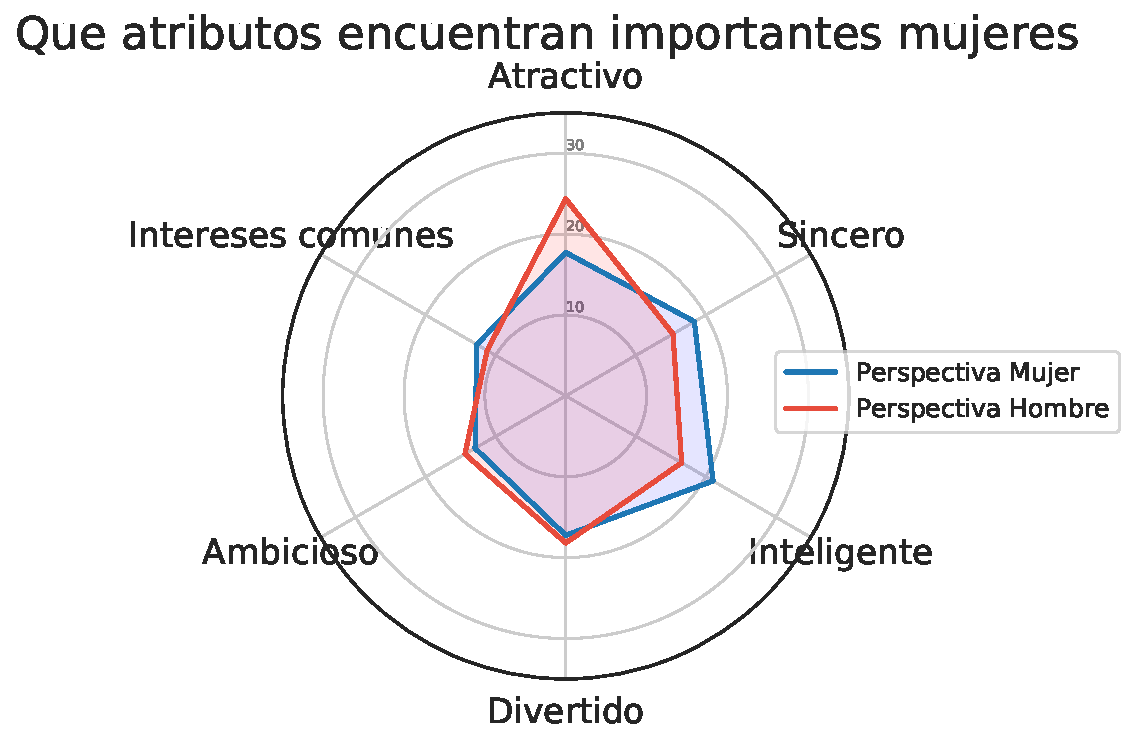
\includegraphics[width=.95\linewidth]{images/attr_females.pdf}
  \captionof{figure}{Promedio de la encuesta sobre que atributos son importantes para las mujeres, según punto de vista de mujeres y hombres.}
  \label{im:f_seek_m}
\end{minipage}%
\begin{minipage}{.5\textwidth}
  \centering
  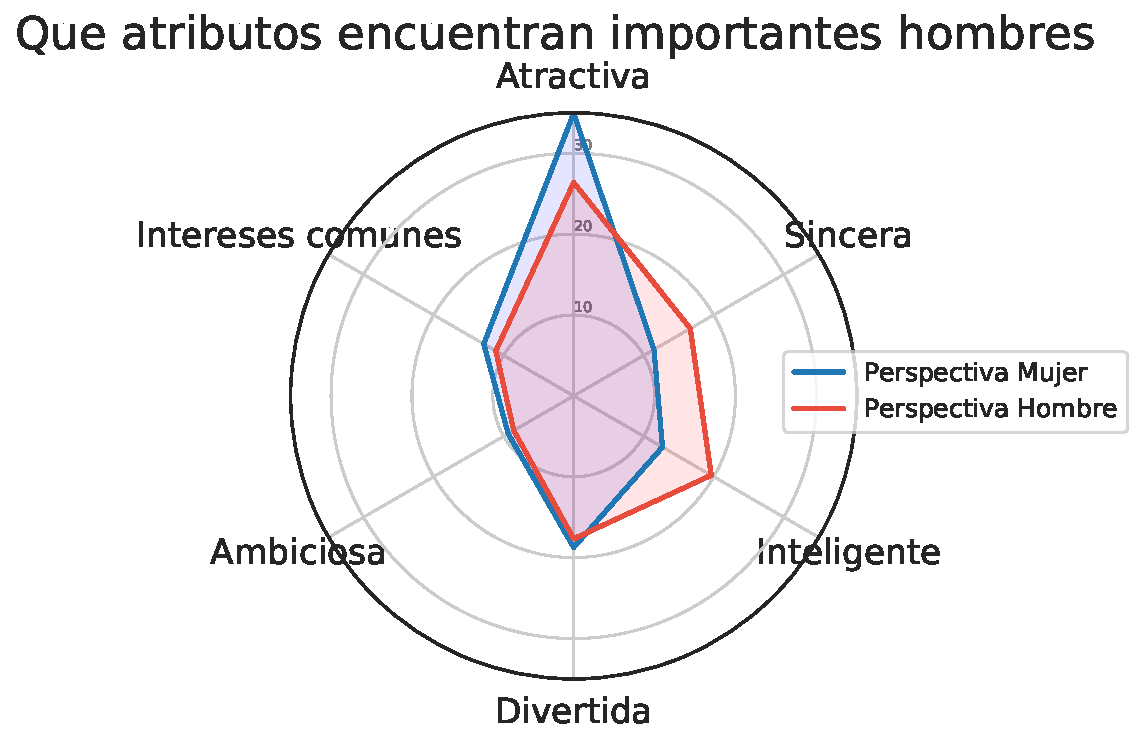
\includegraphics[width=.95\linewidth]{images/attr_males.pdf}
  \captionof{figure}{Promedio de la sobre que atributos son importantes para las hombres, según punto de vista de hombres y mujeres.}
  \label{im:m_seek_f}
\end{minipage}
\end{figure}


Otro punto importante que esta incluido en la encuesta es como cada persona se auto-valora en estos atributos, en este caso solo serían cinco pues intereses comunes no es algo auto-valorable. Con esto y la valoración que entrega cada participante sobre su pareja es posible estudiar la discrepancia entre como alguien se auto-percibe versus como lo perciben los demás. Para esto es de notar que en la pregunta de valorar a tu pareja, un porcentaje pequeño de gente fue capaz de asignar una valor a la ambición de la otra persona, posiblemente dado que es un concepto un poco más abstracto que los otros, y que en solo cuatro minutos no es posible conocer de forma profunda a una persona, es por esto que no se muestra la diferencia en este campo.

En la fig.\ref{im:selfrate} se muestra la distribución de la diferencia entre ($valoracion_{propia} - valoracion_{demas}$) separados por sexo. Valores negativos en la distribución quiere decir una sub-valoración del atributo, es decir que la auto-percepción es más baja de lo que en general opina el sexo opuesto. Con esto podemos ver que en general la auto-percepción es relativamente acertada, con la mediana cerca de $0$, en cuanto a diferencias de cada género, podemos ver que la distribución de atributos en mujeres tiende a tener colas pesadas en valores positivos, lo que quiere decir que se consideran con un atributo más alto de lo que los hombres piensan de ellas. También se aprecia que la media de la distribución para los hombres es un poco más baja que para las mujeres sugiriendo una sub-valoración, esto es más notorio en el caso del atractivo.

\insertimage[\label{im:selfrate}]{diff_distr.pdf}{width=0.45\linewidth}{Distribución de la diferencia entre la auto-valoración de atributos frente a como los demás valoran. La diferencia es obtenida como (auto-percepción $-$ percepción-pareja) por lo que un valor negativo en la distribución es sub-autovaloración mientras que positivos son sobre-autovaloración. Mujer$=0$ Hombre$=1$.}


\subsection{Modelos}
Una vez que se tiene una idea general de como distribuyen las variables, se decide intentar predecir tres escenarios: (i) utilizando solo como valoran a su pareja, si tienen la misma raza, correlación de intereses y genero, poder predecir si esa persona desea seguir con una segunda cita, (ii) dado las mismas variables predecir cuanto le gusta a la persona su pareja, en una escala de $0$ a $10$, por último (iii) utilizando la valoración mutua que tiene una pareja (es decir como ella lo valora a él y él a ella en los 6 atributos) junto con intereses correlacionados, y si se tiene la misma raza, poder predecir finalmente un match. Desde ahora se referirá como atributos a los $4$ atributos: Atractivo, sinceridad, inteligencia y humor. Ambición se descartó por falta de respuestas en la encuesta y los intereses mutuos se obtienen mediante la correlación entre respuestas de preferencias de pasatiempos por cada uno.

Es de notar que fueron usadas pocas variables respecto al número inicial de la base de datos, esto se debe a que las demás variables o eran redundancias como volver a incluir preferencia de atributos, o eran variables que no deberían tienen relación de la persona sobre un match, un ejemplo de esto es la variable que dice cuan feliz o satisfecho se está con el experimento total, o si logró establecer una conexión luego de la segunda cita. Es de mencionar que $17$ variables correspondiente a gustos independientes de cada personas respecto a hobbies y actividades quedan condensados en la correlación entre intereses.

Para cada experimento se ajustaron tres modelos: Descision Tree, Random Forest y XGBOOST. Donde el primer y tercer experimento corresponden a modelos de clasificación y el segundo de regresión. Todos los modelos fueron entrenados con los mismos datos realizando una partición de entrenamiento y test de $2/3$ y $1/3$ respectivamente.


\textbf{Predicción de decisión}: para el primer experimento se quiere intentar predecir si, dado la información que tiene la persona de su pareja, va a decidir querer una segunda cita o no, esto es independiente de qué decide la otra persona. Para esto se usan $7$ predictores, los primeros $4$ es como califica a su cita en los cuatro atributos junto a esto se suma correlación intereses comunes, una variable binaria que indica que ambos pertenecen a la misma raza y por último el género. El género se incluye puesto que al utilizar árboles se espera que si existe diferencia en la forma de tomar decisión para hombres y mujeres, una rama del árbol permite que se modele esta diferente y así evitar ajustar dos modelos diferentes por genero.


\textbf{Regresión de gusto}: usando los mismos atributos que en caso anterior, se busca predecir cuanto le gusta a un participante su cita, en una escala de $0$ a $10$.

\textbf{Predicción de match}: Usando ahora la calificación de ambas partes respecto a los $atributos$ y descartando el uso de género pues ahora se quiere clasificar una cita en vez de la opinión de una persona, se tienen $10$ variables para predecir un match, que es cuando ambas personas dicen sí al primer experimento.

Luego, para cada experimento cada modelo (clasificador o regresor según el caso) fue entrenado bajo $100$ inicializaciones distintas, a fin de tener más robustez en el resultado, en el caso de Random Forest y XGBOOST ambos fueron entrenados en cada caso con $n=50$ árboles. Como métrica de comparación se utilizo el \textit{accuracy} promedio en los casos de clasificación y el error absoluto medio promedio (MAE) para el caso de regresión.
En la tabla.\ref{tab:tree_results} se muestra el resultado de los $100$ intentos, para cada modelo, para cada experimento.

\begin{table}[h!]
\centering
\begin{tabular}{l l l}
\toprule
Experimento & Modelo & Rendimiento\\ 
\midrule
\multirow{3}{*}{Clasificación sobre decisión} & Decision Tree & $0.655 \pm 3.063 \cdot 10^{-03}$ \\
                                              & Random Forest & $0.705 \pm 4.048 \cdot 10^{-03} $ \\ 
                                              & XGBOOST & $\mathbf{0.735 \pm 1.443 \cdot 10^{-15}}$ \\
\midrule
\multirow{3}{*}{Regresión sobre gusto} & Decision Tree & $1.192 \pm 6.509 \cdot 10^{-03}$  \\
                                       & Random Forest & $0.913 \pm 3.905 \cdot 10^{-03}$\\
                                       & XGBOOST & $\mathbf{0.845 \pm 1.221 \cdot 10^{-15}}$ \\
\midrule
\multirow{3}{*}{Clasificación sobre Match} & Decision Tree & $0.768  \pm  4.216 \cdot 10^{-03}$ \\
                                           & Random Forest & $0.843 \pm 2.864 \cdot 10^{-03}$ \\
                                           & XGBOOST & $\mathbf{0.853 \pm 9.992 \cdot 10^{-16}}$ \\
\bottomrule
\end{tabular}
\caption{Métricas de rendimiento en el conjunto de test para los $3$ experimentos con $100$ intentos por cada modelo, por cada experimento. Se muestra la media de la métrica de rendimiento y la desviación estándar para los $100$ instancias. Se usa Accuracy promedio para los problemas de clasificación y MAE promedio para el de regresión. En negrita se muestra el mejor modelo por experimento}
\label{tab:tree_results}
\end{table}


Respecto al primer experimento, se puede ver que el mejor modelo es XGBOOST que alcanza un accuracy promedio del $73\%$ y una desviación estándar pequeña, indicando que el modelo consistentemente es capaz de predecir si una persona decidirá preguntar por una segunda cita.

Para la regresión sobre cuanto le gusta a una persona su cita, podemos ver que nuevamente XGBOOST es el que tiene mejor desempeño con un error absoluto medio de cercano a $0.8$ en una escala de $0$ a $10$, es interesante estudiar como se relaciona cuanto le gusta a una persona con la decisión de preguntar por la segunda cita. Es de esperar que exista al menos una correlación positiva, lo cual empíricamente no se encuentra ya que, (i) no existe correlación entre cuanto le gusta una persona con la decisión de preguntar con la segunda cita, (ii) la adición de esta variable como predictor no mejora el rendimiento de los modelos ni en el segundo ni tercer experimento.

Finalmente en el tercer experimento, en donde se quiere predecir un match, XGBOOST termina por ser el mejor modelo, siendo capaz de predecir un match con un $85\%$ de accuracy para el conjunto de test y con una desviación estándar varios ordenes de mágnitud menores al de Random Forest.


\subsection{Ranking variables}
Por último, dado que los modelos son capaces de consistentemente predecir tanto una decisión unilateral como un match, se busca en cada caso comparar el ranking de atributos intrinseco dado por los modelos basados en árboles. Para esto, por cada experimento se toma el último modelo entrenado y se evalúa el ranking de características, dado en los tres modelos por la perdida promedio por variable de la función objetivo del árbol, índice gini en el caso de clasificación y error cuadrático medio en el de regresión.

\textbf{Clasificación de decisión}: Se muestra en las fig.\ref{im:exp1_dt} fig.\ref{im:exp1_rf} y fig.\ref{im:exp1_xgb} el ranking de variables para Decision Tree (DT), Random Forest (RF) y XGBOOST (XGB) respectivamente. En estos se puede ver que en DT y RF los atributos más importantes parecen ser en primer lugar los intereses comunes y en segundo el atractivo, mientras que en XGB es altamente preponderante el atractivo y lejano aparece el humor.

Es interesante notar que el género no resulta ser una variable decisiva en la decisión, lo cual índica que la forma en que se toman las decisiones no varia mucho entre hombres y mujeres.

\insertimage[\label{im:exp1_dt}]{exp1_dt.pdf}{width=0.45\linewidth}{Ranking atributos para Decision Tree en clasificación de decisión.}

\insertimage[\label{im:exp1_rf}]{exp1_rf.pdf}{width=0.45\linewidth}{Ranking atributos para Random Forest en clasificación de decisión.}

\insertimage[\label{im:exp1_xgb}]{exp1_xgb.pdf}{width=0.45\linewidth}{Ranking atributos para XGBOOST en clasificación de decisión.}

\textbf{Regresión Gusto}: Siguiendo el mismo análisis, en las fig.\ref{im:exp2_dt} fig.\ref{im:exp2_rf} y fig.\ref{im:exp2_xgb} se muestra el ranking de atributos para la regresión sobre cuanto le gusta su pareja, en este podemos ver que en los tres modelos el humor muestra ser el atributo más importante. Lamentablemente el gusto no parece estar relacionado con hacer match, por lo que no se puede concluir mucho.

\insertimage[\label{im:exp2_dt}]{exp2_dt.pdf}{width=0.45\linewidth}{Ranking atributos para Decision Tree en regresión gusto.}

\insertimage[\label{im:exp2_rf}]{exp2_rf.pdf}{width=0.45\linewidth}{Ranking atributos para Random Forest en regresión gusto.}

\insertimage[\label{im:exp2_xgb}]{exp2_xgb.pdf}{width=0.45\linewidth}{Ranking atributos para XGBOOST en regresión gusto.}

\textbf{Clasificación Match}: Finalmente se tienen los ranking de atributos el clasificación de match en las fig.\ref{im:exp3_dt} fig.\ref{im:exp3_rf} y fig.\ref{im:exp3_xgb}. Para el caso de DT y RF se ve que los intereses comunes juegan un rol importante en la clasificación quedando en segundo lugar atractivo y humor. Sin embargo en el caso de XGBOOST el atractivo y humor quedan en primer lugar. En los tres casos es de notar que como existen dos variables asociadas a los atributos (pues se esta viendo la percepción del uno del otro en la cita) y se puede ver que mismos atributos tienen ranking similares para todos los modelos, lo cual muestra consistencia.

El resultado de este último ranking es llamativo al contrastarlo con la valoración de atributos que se busca en la otra persona mostrado en las fig.\ref{im:f_seek_m} y fig.\ref{im:m_seek_f} donde la inteligencia y sinceridad mostraban ser los atributos predominantes en ambos casos. Esto contrasta directamente con lo obtenido en los modelos, donde el sentido del humor y el atractivo muestran ser los factores más predominantes a la hora de tomar la decisión. Una explicación de esto puede ser que, como la citas solo toman cuatro minutos, este tiempo no es suficiente para evaluar la inteligencia y sinceridad del otro, y la decisión debe ser tomada frente a atributos más directos como el atractivo o el sentido del humor al empezar la conversación liviana. Una conclusión puede ser que, si se cuenta con poco tiempo, es mejor usar el sentido del humor que tratar de entablar una conversación profunda!.

Otro punto interesante a notar es que tanto RF como XGB tuvieron desempeños similares a la hora de predecir un match, sin embargo estos usaron variables diferentes para realizar la predicción.


\insertimage[\label{im:exp3_dt}]{exp3_dt.pdf}{width=0.45\linewidth}{Ranking atributos para Decision Tree en clasificación match.}

\insertimage[\label{im:exp3_rf}]{exp3_rf.pdf}{width=0.45\linewidth}{Ranking atributos para Random Forest en clasificación match.}

\insertimage[\label{im:exp3_xgb}]{exp3_xgb.pdf}{width=0.45\linewidth}{Ranking atributos para XGBOOST en clasificación match.}



\section{Conclusión}

Se exploró de forma satisfactoria la base de datos de citas express, pudiendo comparar el comportamiento de hombres y mujeres a la hora de elegir pareja cuando se tiene una restricción de cuatro minutos para entablar la conversación. Todo esto frente a valoraciones y percepciones de cinco atributos: atractivo, sinceridad, ambición e inteligencia. Fue posible entrenar modelos predictivos de forma exitosa y estimar si una pareja hará un match.

Al comparar las diferencias de que parece preferir un genero frente a lo que el otro piensa que prefiere, se puede ver que ambos sexos piensan que el otro valora de sobremanera el atractivo físico, donde en ambos casos se llega a un sobre estimación de la importancia de este atributo. Para mujeres parece ser más importante la inteligencia y sinceridad, mientras que para los hombres el atractivo e inteligencia ocupan los primeros lugares.

Sorprendentemente, la auto-percepción de los participantes frente a estos cinco atributos es en general acertada, donde la mediana de la diferencia entre lo auto-percibido y lo que los demás perciben se centra en $0$. A pesar de esto existen diferencias entre géneros donde mujeres tienen a sobre-estimar sus atributos mientras que hombres tienen a permanecer centrales, con una tendencia muy leve a sub-estimar su propio atractivo.

Respecto a los modelos ajustados, se logro predecir tanto si una persona decide unilateralmente preguntar por una segunda cita, como cuanto le gusta la otra persona como finalmente si se logra un match. Para esto los métodos basados en árboles resultados ser efectivos en rendimiento y al mismo tiempo entregar un ranking sobre que atributo impacta más en la decisión.

Ni el sexo ni la raza jugaron un rol importante en la predicción, lo que da a pensar que no existen muchas diferencias en la forma de tomar la decisión para hombres y mujeres, y que el ser de la misma etnia bajo un contexto universitario tampoco afecta.

Interesante es como cuando es preguntado la importancia de cada atributo, la inteligencia y sinceridad en el caso de las mujeres, y atractivo e inteligencia en el caso de los hombres parecen ser los factores decisivos, sin embargo en el caso de ser citas express de cuatro minutos, el humor y el atractivo terminan siendo los factores importantes, sin importar el género. Una explicación es que el corto tiempo que se tiene para hablar con la persona no permite evaluar conceptos más complejos como la inteligencia y sinceridad.

% \insertimage[\label{im:cart}]{cart.PNG}{scale=0.5}{ Diagrama de cuerpo libre del carro [Enunciado de la actividad].}



% \begin{table}[h!]
% \centering
% \begin{tabular}{c c c c}
% \toprule
% Estado & Overshoot [$\%$] & {Tiempo Establecimiento [s]} & \\ 
% \midrule
% $x_{fenom}$ & 16.289 & 2.512 \\ 
% $x_{lin}$ & 16.385 & 2.544 \\
% $\varphi_{fenom}$ & 52.466 & 3.148 \\
% $\varphi_{lin}$ & 51.309 & 3.145 \\
% \bottomrule
% \end{tabular}
% \caption{Métricas LQR sin ruido ni observador.}
% \label{tab:lqr_results}
% \end{table}


% \begin{thebibliography}{10}

\bibliography{ref}
% \bibitem{eolica}        
%      Quintanilla, S.
%     \textit{La eólica en el mundo | Asociación Empresarial Eólica.}
%     \\ \url{https://www.aeeolica.org/es/sobre-la-eolica/la-eolica-en-el-mundo/}
%     \\ Accessed 2 Dec. 2017

% \bibitem{paper}
%     David Siegel \& Jay Lee.
%     \\ \textit{ An Auto-Associative Residual Processing and K-means Clustering
%     Approach for Anemometer Health Assessment.}
%     {International Journal of Prognostic and Health Management.}

% \bibitem{phm} PHM Data Challenge 2011
%     \\ \textit{ Condition Monitoring of Anemometers.}
%      { PHM Society.}
        
% \end{thebibliography}


% \newpage

% \newtitleanum{Anexos}

\section{Anexos}

\insertimage[\label{im:diagramalineal}]{exp2_pendulo_LQR.pdf}{width=0.7\linewidth}{Diagrama de bloques \textit{Simulink} para modelo lineal y modelo no lineal.}


\insertimage[\label{im:simulink_obs1}]{exp2_pendulo_LQR_observer.pdf}{page=1, width=0.7\linewidth}{Implementación \textit{Simulink} sistema lineal y no lineal con observador.}

\insertimage[\label{im:simulink_obs2}]{exp2_pendulo_LQR_observer.pdf}{page=2, width=0.7\linewidth}{Subbloque planta No lineal \textit{Simulink} sistema lineal y no lineal con observador.}

\insertimage[\label{im:simulink_obs3}]{exp2_pendulo_LQR_observer.pdf}{page=3, width=0.7\linewidth}{Subbloque observador lineal \textit{Simulink} sistema lineal y no lineal con observador.}

\insertimage[\label{im:simulink_obs4}]{exp2_pendulo_LQR_observer.pdf}{page=4, width=0.7\linewidth}{Subbloque observador No lineal \textit{Simulink} sistema lineal y no lineal con observador.}

% \begin{figure}[H]
%     \centering
%     \includegraphics[page=1, width=0.99\linewidth]{images/exp2_pendulo_LQR_observer.pdf}
%     \label{im:simulink_obs1}
%     \caption{Implementación \textit{Simulink} sistema lineal y no lineal con observador.}
% \end{figure}

% \begin{figure}[H]
%     \centering
%     \includegraphics[page=2, width=0.99\linewidth]{images/exp2_pendulo_LQR_observer.pdf}
%     \label{im:simulink_obs2}
%     \caption{Subbloque planta No lineal \textit{Simulink} sistema lineal y no lineal con observador.}
% \end{figure}

% \begin{figure}[H]
%     \centering
%     \includegraphics[page=3, width=0.99\linewidth]{images/exp2_pendulo_LQR_observer.pdf}
%     \label{im:simulink_obs3}
%     \caption{Subbloque observador lineal \textit{Simulink} sistema lineal y no lineal con observador.}
% \end{figure}

% \begin{figure}[H]
%     \centering
%     \includegraphics[page=4, width=0.99\linewidth]{images/exp2_pendulo_LQR_observer.pdf}
%     \label{im:simulink_obs4}
%     \caption{Subbloque observador No lineal \textit{Simulink} sistema lineal y no lineal con observador.}
% \end{figure}




% \insertimage[\label{im:simulink_obs}]{exp2_pendulo_LQR.pdf}{width=0.7\linewidth}{Implementación en \textit{Simulink} de observadores de estado.}

% \lstset{style=Python}
% \lstinputlisting[language=python, basicstyle=\fontsize{9}{9}\ttfamily, caption={Implementación 
% preprocesamiento.}]{cod/data_cleaning_paper.py}


% \lstset{style=C}
% \lstinputlisting[language=C, basicstyle=\fontsize{9}{9}\ttfamily, caption={Código completo de la implementación.}]{cod/tarea6.c}

% \lstinputlisting[language=C, basicstyle=\fontsize{9}{9}\ttfamily, caption={\textit{header} con el prototipo.}]{cod/func.h}

% \lstset{style=python}
% \lstinputlisting[language=python,basicstyle=\tiny, caption={Código para hacer las comparaciones entre algoritmos en secuencias aleatorias, ascendentes y descendentes.}]{cod/order_measure.java}


%\begin{figure}[H] \centering
%\begin{subfigure}{.75\textwidth}
%  \centering
%  \includegraphics[width=.75\linewidth]{images/varpar/acceptedRansac_c5.jpg}
%  \caption{$err_{min}=60$, $cons_{min}=5$, $n_{trials}=10000$.}
%  \label{fig:an111}
%\end{subfigure}\\%
%\begin{subfigure}{.75\textwidth}
%  \centering
%  \includegraphics[width=.75\linewidth]{images/varpar/acceptedRansac_c50.jpg}
%  \caption{$err_{min}=60$, $cons_{min}=50$, $n_{trials}=10000$.}
%  \label{fig:an112}
%\end{subfigure}
%\caption{RANSAC: Variación de $umbralcons$.}
%\label{fig:an11_}
%\end{figure}




% FIN DEL DOCUMENTO
\end{document}